\chapter{随机热机}
\section{随机热力学}

\section{随机热机模型}

\section{绝热捷径}


\qquad 在有限时间热力学中,一个非常重要的议题是如何实现不同平衡态的相互转换。因为\textbf{有限时间}的限制使得我们不能够使用准静态的方法,而绝热捷径\cite{Chen2010}提供了这样一种可以在有限时间内实现平衡态转化的策略。这个策略是由 Demirplak and Rice \cite{Demirplak2003}和 Berry \cite{Berry2009} 独立发展出来的。在这个策略提出以后的很长一段时间里,它引起了一大批研究者的关注。下面我们回顾一下绝热捷径是怎么实现的。


\subsection{绝热捷径的实现}


\qquad 考虑量子力学中的绝热定理\cite{Griffiths2018}:如果一个系统的哈密顿量$H_0(t)$随时间变化很缓慢,即$\tau_\mathrm{e} \gg \tau_\mathrm{i}$,其中$\tau_\mathrm{e}, \tau_\mathrm{i}$分别表示环境的特征时间和系统的内部特征时间。那么如果系统在时间$t=0$处于$H_0 (0)$的本征态,即系统的初态$| \psi(0) \rangle = | n(0) \rangle$,绝热定理告诉我们系统在$t$时刻会处于$H_0 (t)$的对应于瞬时本征态$| n(0) \rangle$,并且
\begin{equation}
    |\psi(t)\rangle=|n(t)\rangle e^{i \theta_{n}(t)} e^{i \gamma_{n}(t)}
    \label{eq2.1}
\end{equation}

其中$\theta_{n}(t)=-\frac{1}{\hbar} \int_{0}^{t} E_{n}(t^{\prime}) \M{d} t^{\prime}, \gamma_{n}(t)=i \int_{0}^{t}\langle n(t^{\prime}) | \partial_{t^{\prime}}n(t^{\prime})\rangle \M{d} t^{\prime}$

不难注意到,绝热定理实现了$H_0(t)$的对应的本征态之间的转化$| n(0) \rangle \to | n(t) \rangle$。现在我们考虑取消$\tau_\mathrm{e} \gg \tau_\mathrm{i}$的要求。

假设存在一个哈密顿量$H(t)$,它使得系统的态的演化严格为$|\psi(t)\rangle=|n(t)\rangle e^{i \theta_{n}(t)} e^{i \gamma_{n}(t)}$,则根据薛定谔方程有
\begin{equation}
    i \hbar \PP{}{t} |\psi(t)\rangle= H(t) |\psi(t)\rangle
    \label{eq2.2}
\end{equation}

将\eqref{eq2.1}代入\eqref{eq2.2},整理得$ E_{n}+ i \hbar \left( | \partial_{t} n \rangle -\langle n | \partial_t n \rangle\right)|n\rangle=H| n\rangle$,于是可得
\begin{equation}
    \begin{split}
        H(t)&=H_{0}(t)+i \hbar \sum_{m}\left(\left|\partial_{t} m\right\rangle\left\langle m\left|-\left\langle m \mid \partial_{t} m\right\rangle\right| m\right\rangle\langle m|\right) \\
        &\equiv H_0 + H_1
    \end{split}
    \label{eq2.3}
\end{equation}
于是一个以$H (t)$作为哈密顿量的系统,若其初态为$H_0 (t)$的本征态$| n(0) \rangle$,那么不论$H (t)$随时间的变化快慢与否,在$t$时刻,系统的状态依然是$H_0 (t)$的本征态,只是两者有一个相位差。于是我们实现了在有限时间内的本征态之间的转化。这其中的关键在于我们引进了一个\textbf{反绝热哈密顿量}$H_1 (t)$,根据\eqref{eq2.3},我们已经在形式上得到了$H_1 (t)$。现在我们考虑对于具体的$H_0 (t)$,如何得到$H_1 (t)$的具体表达式。\cite{Jarzynski2013}

让$H_0$通过一系列参数$\bm{\lambda}(t)=\left( \lambda_1 (t) , \lambda_1 (t) , \lambda_1 (t) , \cdot , \lambda_{N} (t) \right)$依赖于时间$t$。同时,$H_0 (\bm{\lambda})$的本征值、本征态为$E_n (\bm{\lambda}), | n (\bm{\lambda}) \rangle$,根据复合函数的微分法则,式\eqref{eq2.4}可以写为
\begin{equation}
    H_1 (t)=\dot{\boldsymbol{\lambda}} \cdot \boldsymbol{\xi}(\boldsymbol{\lambda}(t))
    \label{eq2.5}
\end{equation}
其中
\begin{equation}
    \boldsymbol{\xi}(\boldsymbol{\lambda})=i \hbar \sum_{m}(|\boldsymbol{\nabla} m\rangle\langle m|-\langle m \mid \boldsymbol{\nabla} m\rangle| m\rangle\langle m|)
    \label{eq2.4}
\end{equation}
同时$|\nabla m\rangle \equiv \partial_{\boldsymbol{\lambda}}|m(\boldsymbol{\lambda})\rangle  , \dot{\boldsymbol{\lambda}} \equiv \mathrm{d} \lambda / \mathrm{d} t$

把$\boldsymbol{\xi}$看做参数空间的无穷小平移$\boldsymbol{\lambda} \to \boldsymbol{\lambda} + \delta \boldsymbol{\lambda}$的生成元。这个无穷小平移与希尔伯特空间中态的变换$|\psi\rangle \rightarrow|\psi\rangle+|\delta \psi\rangle$相联系,通过以下方式
\begin{equation}
    i \hbar|\delta \psi\rangle=\delta \boldsymbol{\lambda} \cdot \boldsymbol{\xi}|\psi\rangle
    \label{eq2.6}
\end{equation}
这样,在一阶近似下,$H_0 (\bm{\lambda})$的本征态$|n(\bm{\lambda})\rangle$的变换为
\begin{equation}
    |n(\boldsymbol{\lambda})\rangle \rightarrow\left(1+\frac{1}{i \hbar} \delta \boldsymbol{\lambda} \cdot \hat{\boldsymbol{\xi}}\right)|n(\boldsymbol{\lambda})\rangle=e^{i \delta \boldsymbol{\lambda} \cdot \boldsymbol{A}_{n}}|n(\boldsymbol{\lambda}+\delta \boldsymbol{\lambda})\rangle
    \label{eq2.7}
\end{equation}
其中$\boldsymbol{A}_{n}(\boldsymbol{\lambda})=i\langle n | \boldsymbol{\nabla} n\rangle.$ 这意味着,沿着参数空间的曲线$\bm{\lambda}$利用式\eqref{eq2.7},可以将系统的态逐步从$|n(\M{\lambda_0})\rangle$变换成$\M{e}^{i \int_{\bm{\lambda_0}}^{\bm{\lambda_s}}   i\langle n | \boldsymbol{\nabla} n\rangle \M{d}\bm{\lambda}}\left|n\left(\boldsymbol{\lambda}_{s}\right)\right\rangle.$ 这正是们所希望得到的形式。

现在看看系统态的时间演化,先考虑系统经过一个无穷小时间$\delta t$,则态$|\psi \rangle$将演化为
\begin{equation}
     \left(1+\frac{1}{i \hbar} H \delta t\right)|\psi\rangle=|\psi\rangle+\frac{1}{i \hbar} \delta t H_{0}|\psi\rangle+\frac{1}{i \hbar} \delta \boldsymbol{\lambda} \cdot \boldsymbol{\xi}|\psi\rangle
   \label{eq2.8}
\end{equation}

如果考虑态$|\psi \rangle = |n(\bm{\lambda}) \rangle$,那么\eqref{eq2.8}的物理意义是明显的。$H_0$产生了我们熟悉的动力学相位,而$\boldsymbol{\xi}$产生了几何相因子。

由\eqref{eq2.4}定义的$\bm{\xi}$,也可由下式\eqref{eq2.9}定义,(二者的等价性可由$\langle m \mid \boldsymbol{\nabla} n\rangle=\left\langle m\left|\boldsymbol{\nabla} \hat{H}_{0}\right| n\right\rangle /\left(E_{n}-E_{m}\right)$\cite{Berry2009}加以证明)
\begin{subequations}
    \begin{align}
        \left[ \boldsymbol{\xi}, H_{0} \right] &= i \hbar \left( \boldsymbol{\nabla} H_{0}-\operatorname{diag} \left(\boldsymbol{\nabla} H_{0} \right) \right) \label{eq2.9a}\\
        \langle n|\boldsymbol{\xi}| n\rangle &= 0 \label{eq2.9b}
    \end{align}
    \label{eq2.9}
\end{subequations}
其中$\operatorname{diag}\left(\boldsymbol{\nabla} H_{0}\right)=\sum_{m}|m\rangle\left\langle m\left|\boldsymbol{\nabla} H_{0}\right| m\right\rangle\langle m|.$ 对\eqref{eq2.9a}两端同时进行操作$\langle m|\cdots| n\rangle$,得到$\langle m| \boldsymbol{\xi} | n\rangle (E_n - E_m) = \langle m|i \hbar \left( \boldsymbol{\nabla} H_{0}-\operatorname{diag} \left(\boldsymbol{\nabla} H_{0} \right) \right)| n\rangle$. 可见,\eqref{eq2.9a}决定了$\boldsymbol{\xi}$的非对角元,\eqref{eq2.9b}决定了其非对角元。

式\eqref{eq2.9}提供了一种在经典力学中找到\textbf{反绝热哈密顿量}的对应方法。因为我可以利用量子与经典的对应$[A, B]/i \hbar \to \{A, B\}  $将\eqref{eq2.9}转换为经典的,进而可以在经典力学中找到对应的\textbf{反绝热哈密顿量}。现在考虑一个经典系统,其自由度为1,哈密顿量为$H_0 (\bm{\eta};\bm{\lambda}).$ 其中$\bm{\lambda}$依然为依赖于时间的一系列参数,$\bm{\eta}=(q,p)$为广义坐标和广义动量,确定了相空间的一个点。对于确定的能量$E = H_0 (\bm{\eta};\bm{\lambda})$,这将相点约束在相空间的一个能壳上,积分
\begin{equation}
    I(E, \boldsymbol{\lambda}) \equiv \int \mathrm{d} \bm{\eta} \theta\left[E-H_{0}(z ; \boldsymbol{\lambda})\right]
  \label{eq2.10}
\end{equation}
表示的是能壳所围成的体积,阶跃函数$\theta\left[E-H_{0}(z ; \boldsymbol{\lambda})\right]$可以使得积分区域为整个相空间。经典的绝热定理告诉我们$I(E, \boldsymbol{\lambda})$是一个\textbf{绝热不变量} \cite{LiuChuan2019}。也就是说如果$H_0$随时间$t$变化的足够缓慢,那么能壳所围成的体积将保持不变。定义任意可观测量$A$的\textbf{微正则分布平均}
\begin{equation}
    \langle A \rangle_{E, \lambda} \equiv \frac{1}{\partial_{E} I} \int \mathrm{d} \bm{\eta} \delta\left(E-H_{0}\right) A
  \label{eq2.11}
\end{equation}
利用函数$I (E,\bm{\lambda})$去定义函数$E (I, \bm{\lambda})$,则有
\begin{equation}
    \boldsymbol{\nabla} E(I, \boldsymbol{\lambda})=-\frac{\boldsymbol{\nabla} I(E, \boldsymbol{\lambda})}{\partial_{E} I(E, \boldsymbol{\lambda})}=\left\langle\boldsymbol{\nabla} H_{0}\right\rangle_{E, \boldsymbol{\lambda}}
  \label{eq2.12}
\end{equation}
其中第一个等式利用循环函数的偏导数的性质,第二个等式利用了式\eqref{eq2.10}和式\eqref{eq2.11}。

式\eqref{eq2.9}的经典对应为\cite{Jarzynski1995}
\begin{subequations}
    \begin{align}
        \left\{\boldsymbol{\xi}, H_{0}\right\} &=\boldsymbol{\nabla} H_{0}-\left\langle\boldsymbol{\nabla} H_{0}\right\rangle_{E, \boldsymbol{\lambda}} \equiv \boldsymbol{\nabla} \tilde{H}_{0}    \label{eq2.13a}\\
        \langle\boldsymbol{\xi}\rangle_{E, \boldsymbol{\lambda}} &=0 \label{eq2.13b}
    \end{align}
    \label{eq2.13}
\end{subequations}
其中$\{ \cdots \}$是经典力学中的泊松括号$\{A, B\}=(\partial A / \partial q)(\partial B / \partial p)-(\partial A / \partial p)(\partial B / \partial q)$。利用式\eqref{eq2.12}和泊松括号的定义,式\eqref{eq2.13a}可改写为\R{不懂,出自\cite{Jarzynski2013} page2 (13)}
\begin{equation}
    \{\boldsymbol{\xi}, i\}=\boldsymbol{\nabla} i
  \label{eq2.14}
\end{equation}
其中关于$\bm{\eta}$和$\bm{\lambda}$的函数$i$的定义为:$i (\bm{\eta}; \bm{\lambda}) \equiv I \left( H_0\left( \bm{\eta}; \bm{\lambda}\right) ; \bm{\lambda} \right)$。类似于量子的情形的,将$\boldsymbol{\xi} (\bm{\eta}; \bm{\lambda})$看做和参数空间的无穷小平移$\boldsymbol{\lambda} \to \boldsymbol{\lambda} + \delta \boldsymbol{\lambda}$相联系的相空间的平移$\bm{\eta} \to \bm{\eta} + \delta \bm{\eta}$的生成元,有\cite{H.1986}
\begin{equation}
    \delta \bm{\eta}=\delta \boldsymbol{\lambda} \cdot\{\bm{\eta}, \boldsymbol{\xi}\}
  \label{eq2.15}
\end{equation}
于是,由式\eqref{eq2.14}和\eqref{eq2.15}可得
\begin{equation}
    \begin{split}
        &i(\bm{\eta}+\delta \bm{\eta} ; \boldsymbol{\lambda}+\delta \boldsymbol{\lambda})-i(\bm{\eta} ; \boldsymbol{\lambda}) \\
        =&\frac{\partial i}{\partial \bm{\eta}} \delta \bm{\eta}+\boldsymbol{\nabla} i \cdot \delta \boldsymbol{\lambda} \\
        =&(\{i, \boldsymbol{\xi}\}+\nabla i) \cdot \delta \boldsymbol{\lambda}\\
        =&0
    \end{split}
    \label{eq2.16}
\end{equation}
这说明,变换$\bm{\eta} \to \bm{\eta} + \delta  \bm{\lambda} \cdot \{\bm{\eta}, \boldsymbol{\xi}\}$将能壳$H_{0}(\bm{\eta} ; \boldsymbol{\lambda})$上的一个相点映射到能壳$H_{0}(\bm{\eta} + \delta \bm{\eta} ; \boldsymbol{\lambda})$上的一个点,而二者包围着相同的相体积。

可见,类似于量子中的情形,只要给经典的系统施加一个反绝热的哈密顿量$\dot{\boldsymbol{\lambda}} \cdot \boldsymbol{\xi}(\bm{\eta}, \boldsymbol{\lambda}(t))$。那么此系统的$I(E, \boldsymbol{\lambda}) \equiv \int \mathrm{d} \bm{\eta} \theta\left[E-H_{0}(z ; \boldsymbol{\lambda})\right]$将严格保持不变,不论$H_0 $随时间的变化快慢与否。这个新的哈密顿量为\R{(文献\cite{Jarzynski2013} page eq16直接计算了$\DD{}{t} i (\bm{\eta}; \bm{\lambda})$,但其中的推理过程未能理解)}
\begin{equation}
    H(\bm{\eta}, t)=H_{0}(\bm{\eta} ; \boldsymbol{\lambda}(t))+\dot{\boldsymbol{\lambda}} \cdot \boldsymbol{\xi}(\bm{\eta}, \boldsymbol{\lambda}(t))
    \label{eq2.17}
\end{equation}

\emph{从系综的角度来考虑这个过程:想象一下从H0的能壳E0中取样的初始条件的集合。在任何后来的时间t>0,从这些初始条件演化出来的轨迹,在Hamiltonian H(z; t)下,将填充一个H0(z;(t))的单一能壳E(t),具体来说是绝热能壳,它与初始能壳的相空间体积相同。如果我们把绝热能壳想象成一个随着参数随时间变化而变形的闭合循环,那么在式16中,H0围绕这个循环产生运动,调整每个轨迹,使其保持在壳上。}\R{可不要,出自\cite{Jarzynski2013} page eq16}

\subsection{经典和量子偶次幂势场中生成元的构造}

\qquad 现在,鉴于变换$\bm{\eta} \to \bm{\eta} + \delta  \bm{\lambda} \cdot \{\bm{\eta}, \boldsymbol{\xi}\}$将能壳$H_{0}(\bm{\eta} ; \boldsymbol{\lambda})$ 上的相点映射到了能壳 $ H_{0}(\bm{\eta} + \delta \bm{\eta} ; \boldsymbol{\lambda})$上,我们可以此为根据构造经典力学中的$\boldsymbol{\xi}(\bm{\eta}, \boldsymbol{\lambda})$,下面我们用例子进行说明

考虑一个一维的粒子,处在两堵刚性墙之间,刚性墙的位置为$q=0,\lambda$,这个例子这对应于量子力学中的一维无限深势阱。其相空间的能壳如图\eqref{p2.1}所示。
\begin{figure}[!htbp]
    \begin{center}
        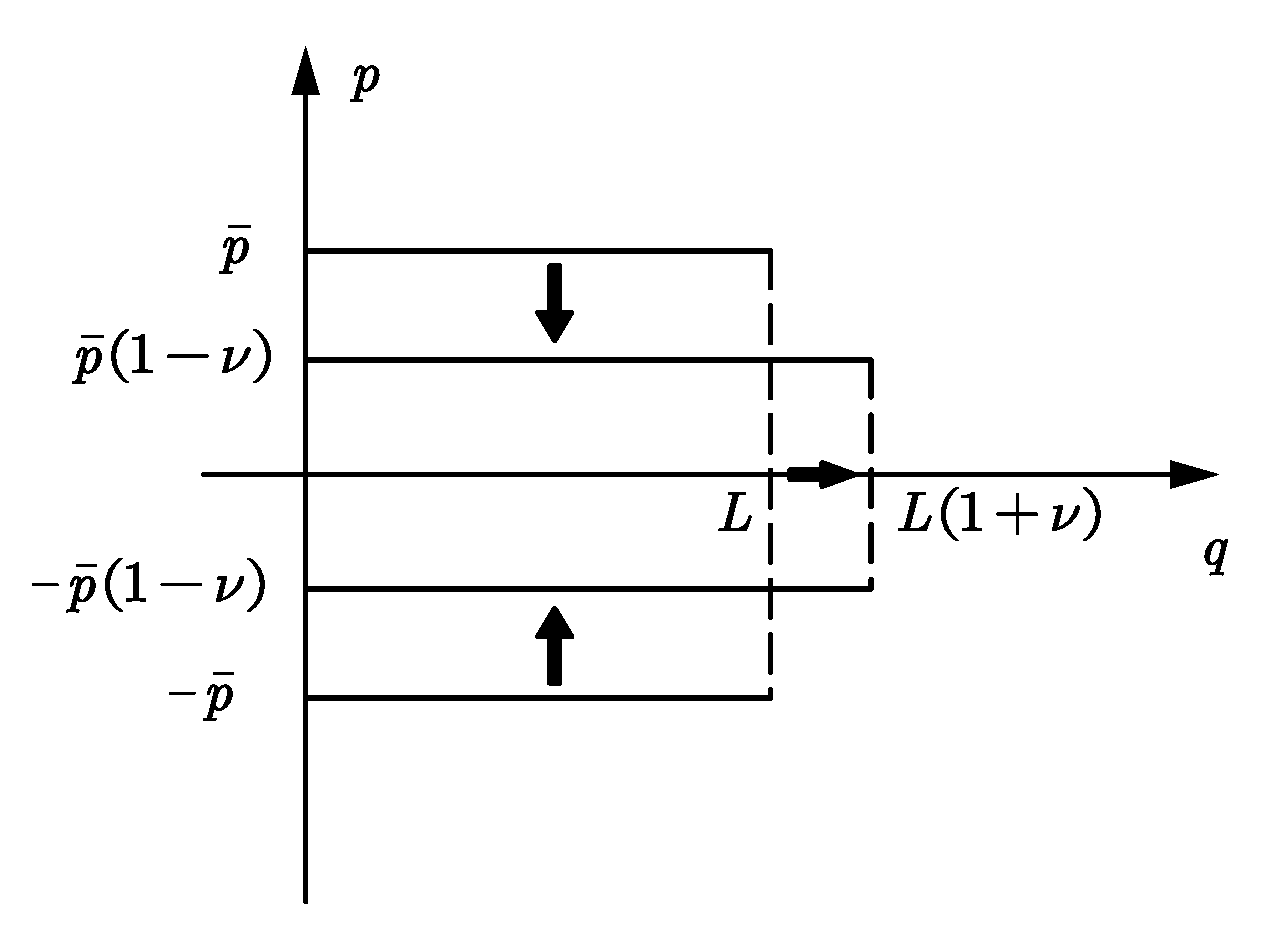
\includegraphics[width=0.5\textwidth]{figures/p2.1.pdf}
    \end{center}
    \caption{在一维盒子中的粒子的能壳。该粒子的能壳是一个矩形,当盒子的长度发生极小的改变时,矩形能壳也发生相应的改变。但矩形的体积不变}
    \label{p2.1}
\end{figure}

系统的哈密顿量为
\begin{equation}
     H_{0}(\bm{\eta} ; \lambda)=\frac{p^{2}}{2 m}+V_{\mathrm{box}}(q ; \lambda)
        \label{eq2.18}
\end{equation}
其中$V_{\mathrm{box}}(q ; \lambda)$代表一维盒子的势场$V_{\mathrm{box}}(q ; \lambda) = \left\{\begin{array}{l} 0 ,\ q<\lambda\\ \infty ,\ q \leq 0\ \text{or}\ q \geq \lambda \end{array}\right.$在经典中这个粒子的运动是平凡的——以相同的速度在两堵墙之间做往返运动。
    
哈密顿量的参数$\lambda$随时间$t$变化,现在我们构造这个系统的\textbf{反绝热哈密顿量}。不难得出,矩形能壳的面积为$I=2 \bar{p} \lambda$,由于矩形能壳的长的变化为$\lambda \to \lambda(1+\nu)$,为了维持矩形能壳的面积,在一阶精度下,可令其宽的微小改变为$2 \bar{p} \to 2 \bar{p} (1-\nu)$,其中$\nu \equiv \delta \lambda / \lambda$。于是,这两个能壳被一个线性的尺度变换所联系
\begin{equation}
    q \rightarrow q(1+\nu) \quad, \quad p \rightarrow p(1-\nu)
    \label{eq2.19}
\end{equation}
现在我们可以通过$(\nu q,\ -\nu p)  = \delta \lambda \{ (q,\ p),\ \xi \}$(式\eqref{eq2.15})逆向解出生成元的表达式,于是我们可得一对这样的方程$\left\{ \begin{array}{l} q / \lambda=\partial \xi / \partial p \\ p / \lambda=\partial \xi / \partial q \end{array}\right.$。结合限制条件\eqref{eq2.13b},于是可令$\xi = q p / \lambda$。再根据式\eqref{eq2.19},我们最终得到
\begin{equation}
    H(\bm{\eta}, t)=H_{0}(\bm{\eta} ; \lambda)+\frac{\dot{\lambda}}{\lambda} q p \quad, \quad \lambda=\lambda(t)
    \label{eq2.20}
\end{equation}
在这个时间依赖的哈密顿量之下,绝热不变量$i(q,\ p;\ \lambda)=2 |p| \lambda$是严格守恒的,不论函数$\lambda(t)$的形式是怎样的。现在我们对于这个具体的例子,实实在在的构造出了\textbf{反绝热哈密顿量},这说明其并不只是存在于形式化理论中,而是可以在实际中加以利用的。

在构造出了经典的\textbf{反绝热哈密顿量}之后,我们也可以通过$\xi$的经典表达式来猜想量子力学中的\textbf{反绝热哈密顿量},因为算符$p,\ q$是不对易的,一个自然的猜想是
\begin{equation}
    \xi(\lambda) = \frac{q p + p q}{2 \lambda}
    \label{eq2.21}
\end{equation}
于是,再联系到已知的量子力学中\textbf{一维无限深势阱}的本征解,非常幸运的,我们发现选择的这个$\xi$满足式\eqref{eq2.7}
\begin{equation}
    \left(1+\frac{1}{i \hbar} \delta \lambda \xi \right) \sqrt{\frac{2}{\lambda}} \sin \left(\frac{n \pi q}{\lambda}\right)=\sqrt{\frac{2}{\lambda+\delta \lambda}} \sin \left(\frac{n \pi q}{\lambda+\delta \lambda}\right)
    \label{eq2.22}
\end{equation}
这一点可以通过计算$\PP{}{\lambda} \sqrt{\frac{2}{\lambda}} \sin \left(\frac{n \pi q}{\lambda}\right) \delta \lambda = \frac{1}{i \hbar} \delta \lambda \xi \sqrt{\frac{2}{\lambda}} \sin \left(\frac{n \pi q}{\lambda}\right)$得到验证。\eqref{eq2.22}中的相位由于$A_{n}(\lambda)=i\langle n | \partial_\lambda  n\rangle = 0$而消失。于是可以立刻得到
\begin{equation}
    H(t)=-\frac{\hbar^{2}}{2 m} \frac{\partial^{2}}{\partial q^{2}}+V_{\mathrm{box}}(q ; \lambda)+\frac{\dot{\lambda}}{2 \lambda} \frac{\hbar}{i}\left(q \frac{\partial}{\partial q}+\frac{\partial}{\partial q} q\right)
    \label{eq2.23}
\end{equation}
这样,波函数
\begin{equation}
    \psi (q, t)=\sqrt{\frac{2}{\lambda}} \sin \left(\frac{n \pi q}{\lambda}\right) \exp \left(-\frac{i}{\hbar} \int_{0}^{t} \mathrm{~d} t^{\prime} \frac{n^{2} \pi^{2} \hbar^{2}}{2 m \lambda^{2}}\right)
    \label{eq2.24}
\end{equation}
将成为这个系统的精确解(初态为$\psi (q,\ 0) = \sqrt{\frac{2}{\lambda}} \sin \left(\frac{n \pi q}{\lambda}\right)$),不论$\lambda(t)$的函数形式如何。

式\eqref{eq2.23}也可以更一般的写成
\begin{equation}
    \left(1+\frac{1}{i \hbar} \delta \lambda \hat{\xi}\right) \psi(q)=\sqrt{\frac{1}{s}} \psi\left(\frac{q}{s}\right) \quad, \quad s=\frac{\lambda+\delta \lambda}{\lambda}
    \label{eq2.25}
\end{equation}
换句话说,算符$\exp (\delta \lambda \xi / i \hbar)$对波函数$\psi(q)$进行了线性放大。(系数$\sqrt{\frac{1}{s}}$保证了波函数的归一化)自此我们也成功的通过构造的\textbf{经典反绝热哈密顿量}构造出了\textbf{量子反绝热哈密顿量}

不难发现,我们的构造能够成功,很大程度上得益于能壳和本征态之间的\textbf{尺度变换}关系能够成立。相似的办法也能够应用于\textbf{偶次幂势场},则经典哈密顿量为
\begin{equation}
    H_{0}(\bm{\eta} ; \lambda)=\frac{p^{2}}{2 m}+\epsilon\left(\frac{q}{\lambda}\right)^{b}
    \label{eq2.26}
\end{equation}
可以证明,对于相应的量子的情形,也是可以按照类似的方式构造其\textbf{量子反绝热哈密顿量}的。其中$\epsilon > 0$调节了能量尺度,而$b$是正偶数。同样的,我们先在经典中加以考虑,再推广到量子中。上述系统的\textbf{绝热不变量}为
\begin{equation}
    \begin{split}
        i(\bm{\eta};\ \lambda) &= 4 \int_0^{\lambda \left(H_0 / \epsilon \right)^{1/b}} \sqrt{2 m \left[ H_0 -\epsilon \left(q/{\lambda}\right)^b\right]} \, \M{d}q \\ 
        &= \sqrt{8 \pi m} \epsilon^{-1 / b} \frac{\Gamma\left(1+\frac{1}{b}\right)}{\Gamma\left(\frac{3}{2}+\frac{1}{b}\right)} \lambda H_0^{\frac{1}{2 \mu}}\\
        &= c \lambda H_0^{\frac{1}{2 \mu}}
    \end{split}
    \label{eq2.27}
\end{equation}
其中,$\mu \equiv \frac{b}{b+2} ,\ c \equiv \sqrt{8 \pi m} \epsilon^{-1 / b} \frac{\Gamma\left(1+\frac{1}{b}\right)}{\Gamma\left(\frac{3}{2}+\frac{1}{b}\right)}$
同样的,含时参数$\lambda \to \lambda + \delta \lambda$的变化,通过一个线性变换引起了能壳的变化。为了看到这一点,我们考虑$i(q,\ p;\ \lambda)$的变化$\delta i(q,\ p;\ \lambda) = \PP{i}{q} \delta q + \PP{i}{p} \delta p + \PP{i}{\lambda} \delta \lambda \equiv 0$,为了使恒等式成立,可以假设$\delta q = x q \frac{\delta \lambda}{\lambda},\ \delta p = - y p \frac{\delta \lambda}{\lambda}$,可以得到
\begin{equation}
    \frac{c}{2 \mu H_0} \left[ (\mu - y) \frac{p^2}{m} + (2 \mu - b + b x) \epsilon \left( \frac{q}{\lambda} \right)^b \right] \delta \lambda \equiv 0
    \label{eq2.28}
\end{equation}
要使上式成立,必须有$x=y=\mu$,可见,能壳的变换依然可以由式\eqref{eq2.19}进行描述,只不过现在$\nu = \mu \delta \lambda / \lambda$,同理我们可以得到新的哈密顿量
\begin{equation}
    H(\bm{\eta}, t)=H_{0}(\bm{\eta} ; \lambda)+\mu \frac{\dot{\lambda}}{\lambda} q p
    \label{eq2.28.5}
\end{equation}
在这个哈密顿量下,$i(\bm{\eta};\ \lambda) = c \lambda H_0^{\frac{1}{2 \mu}}$将成为一个严格的守恒量。在量子力学中,本征态将满足\R{(不甚理解)}
\begin{equation}
    \phi_{n}(q ; \lambda)=\sqrt{\frac{1}{\lambda^{\mu}}} \phi_{n}\left(\frac{q}{\lambda^{\mu}} ; 1\right)
    \label{eq2.29}
\end{equation}
在新的哈密顿量
\begin{equation}
    H(t)=H_{0}(\lambda)+\frac{b}{b+2} \frac{\dot{\lambda}}{2 \lambda} \frac{\hbar}{i}\left(q \frac{\partial}{\partial q}+\frac{\partial}{\partial q} q\right)
    \label{eq2.29.5}
\end{equation}
之下。这结果对任意$b \in \{ 2,\ 4,\ 6,\ \cdots\}$都是成立对的。特别的,$b=2$和$b \to \infty$对应于\textbf{一维谐振子}和\textbf{一维无限深势阱}的情况。不过,对于\textbf{一维谐振子}的情况,Muga等人使用升降算子$a,\ a^{\dagger}$结合式\eqref{eq2.3}的办法更为简单地得到了相同的结果。\cite{Muga2010}

对于一般的一维势场,生成元应该满足
\begin{equation}
    \boldsymbol{\xi}\left(\bm{\eta}_{b} ; \boldsymbol{\lambda}\right)-\boldsymbol{\xi}\left(\bm{\eta}_{a} ; \boldsymbol{\lambda}\right)=\int_{a}^{b} \mathrm{~d} t \nabla \tilde{H}_{0}(\bm{\eta}(t) ; \boldsymbol{\lambda})
    \label{eq2.30}
\end{equation}
其中相点$\bm{\eta}_{a},\ \bm{\eta}_{b}$在同一能壳上,$\bm{\eta}(t)$是相点从$\bm{\eta}_{a}$演化到$\bm{\eta}_{b}$的相轨迹。式\eqref{eq2.30}可以结合式\eqref{eq2.13a}和$(\mathrm{d} / \mathrm{d} t) \boldsymbol{\xi}(\bm{\eta}(t) ; \boldsymbol{\lambda})=\left\{\boldsymbol{\xi}, H_{0}\right\}$而得到。

如果我们考虑相空间中复杂一点的能壳,它们不是简单闭合的环。比如如果势$V(q;\ \bm{\lambda})$是双阱势,而参数$\bm{\lambda}$的变化可以改变能壳的拓扑结构——从单环变成双环或相反。这时$i$的绝热不变性将被破坏。\cite{Tennyson1986,Cary1986,Hannay1986}

对于自由度$f \geq 2$的经典系统,如果$H_0$是\textbf{完全可积的}\cite{LiuChuan2019},我们就有可能能够重复
式\eqref{eq2.10}-\eqref{eq2.17}对\textbf{作用量-角度变量}的分析,每一个生成$\bm{\xi}_i$元对应一对\textbf{作用量-角度变量}。\R{(可加一脚注)}另一个情形下,如果$H_0$是各态历经的,那么式$\eqref{eq2.13a}$的解的存在将意味着能壳$H_0 (\bm{\eta};\ \bm{\lambda})$可以被\textbf{正则变换}到$H_0 (\bm{\eta};\ \bm{\lambda}+\delta \bm{\lambda} )$。\cite{Jarzynski1995}虽然对于$f \geq 2$的系统,这一条件通常并不能满足,但一旦满足,$\bm{\xi}$就简单的是这个变换的生成元,无耗散的驱动就可以由$H_0 + \dot{\boldsymbol{\lambda}} \cdot \boldsymbol{\xi}$实现。

上述的方法除了可以应用在量子和经典动力学之外,相似的方法也可以应用于统计力学,用于估算自由能的变化。其中反绝热的\textbf{度规缩放}\cite{Miller2000}或者\textbf{场流}\cite{Vaikuntanathan2008}被构造出来,用于减少或者消除对有限时间过程中数字模拟的不可逆性。

\subsection{利用绝热捷径实现平衡态的转化}
\qquad 接下来,我们举例说明绝热捷径如何实现平衡态的转化。\cite{Tu2013}考虑一个被时间依赖的谐振子势场驱动的布朗粒子,只需使式\eqref{eq2.26}中的$b=2$,再联系到式\eqref{eq2.29},就可以直接得到它被施加反绝热哈密顿量之后的哈密顿量
\begin{equation}
    \begin{split}
        H(t)=&H_0 (t) + \frac{\dot{\lambda}}{2 \lambda(t)} q p\\
    =&\frac{p^{2}}{2 m}+\epsilon\left(\frac{q}{\lambda}\right)^{2}+\frac{\dot{\lambda}}{2 \lambda(t)} q p
    \end{split}
    \label{eq2.31}
\end{equation}
在时间$t_i < t \leq t_f$内,参数由$\lambda_{i} \equiv \lambda(t_i)$变为$\lambda_{f} \equiv \lambda(t_f)$。我们要求$\dot{\lambda}\left(t_{i}\right)=\dot{\lambda}\left(t_{f}\right)=0$,这样才有$H\left(t_{f}\right)=H_0 \left(t_{f}\right),\ H\left(t_{f}\right)=H_0 \left(t_{f}\right)$,除此之外,$\lambda (t)$依赖于时间$t$的形式有很大的任意性。运动方程为
\begin{equation}
    \left\{\begin{array}{l}
        \dot{q}=\frac{\partial H}{\partial p}=\frac{p}{m}+\frac{\lambda(t)}{2 \lambda(t)} q \\
        \dot{p}=-\frac{\partial H}{\partial q}=-2 \epsilon \frac{q}{\lambda^{2}(t)}-\frac{\dot{\lambda}(t)}{2 \lambda(t)} p
        \end{array}\right.
    \label{eq31.5}
\end{equation}


接下来我们将说明\textbf{绝热捷径}如何联系两个不同\textbf{有效温度}的\textbf{正则态}。\cite{Tu2013}假设系统初始处在有效温度为$\left(k_\M{B} \beta_i\right)^{-1}$的正则态中,那么初始时系统的分布函数可以表达为
\begin{equation}
    \rho_{i}=\frac{\beta_{i}}{2 \pi \lambda_{i}} \exp \left[-\beta_{i} H_0 \left(t_{i}\right)\right]
    \label{eq2.32}
\end{equation}
其中$(q_i,\ p_i)$代表初始时的相点,根据\textbf{刘维尔定理},当系统不和外界任何热浴接触时,分布函数沿着相轨应当是不变的。所以,末态的分布函数应当为
\begin{equation}
    \rho_{f}=\rho_{i}=\frac{\beta_{i} }{2 \pi \lambda_{i}} \exp \left[-\beta_{i} H\left(t_{i}\right)\right]
    \label{eq2.33}
\end{equation}
接着我们寻找末态的有效温度,使得末态的分布函数\eqref{eq2.33}可以被表达成正则分布的样子
\begin{equation}
    \rho_{f}=\frac{\beta_{f} }{2 \pi \lambda_{f}} \exp \left[-\beta_{f} H\left(t_{f}\right)\right]
    \label{eq2.34}
\end{equation}
其中$(q_f,\ p_f)$是末态的相点。计算$H_0 (t)$对时间的导数得
\begin{equation}
    \begin{split}
        \DD{H_0 (t)}{t} =& \frac{p}{m}\dot{p} + 2 \epsilon \frac{q}{\lambda^2}\dot{q} - 2 \epsilon \frac{q^2}{\lambda^2} \dot{\lambda}\\
                        =& -H(t) \DD{\ln{\lambda(t)}}{t}
    \end{split}
    \label{eq2.35}
\end{equation}
第二个等式用到了运动方程\eqref{eq2.34}于是可得$H\left(t_{f}\right)=H\left(t_{i}\right) \lambda_{i} / \lambda_{f}$,将这个式子代入式\eqref{eq2.34},得到
\begin{equation}
    \rho_{f}=\frac{\beta_{f} }{2 \pi \lambda_{f}} \exp \left[-\frac{\beta_{f} \lambda_i}{\lambda_f} H\left(t_{f}\right)\right]
    \label{eq2.36}
\end{equation}
将这个式子和式\eqref{eq2.33}比较可得
\begin{equation}
    \frac{\beta_f}{\lambda_f} = \frac{\beta_i}{\lambda_i}
    \label{eq2.40}
\end{equation}
这说明,如果系统的初态等效温度为$\left( k_\M{B} \beta_i\right)^{-1}$的正则态,那么在系统经历绝热捷径之后,我们可以把系统的末态视为等效温度为$\left( k_\M{B} \beta_f\right)^{-1}$的正则态。而且,初态和末态的等效温度满足\eqref{eq2.40}。

这样,通过绝热捷径,在有限时间时间$t_i \sim t_f$内,我们实现了微观正则态之间的转换。


\section{等温捷径}
    
\qquad 上一节我们介绍了绝热捷径,它可以在有限时间内实现\textbf{正则平衡态}之间的转化。又由于这个过程中,系统和外界没有热交换故而称之为\textbf{绝热捷径}。那么类比于经典中的绝热过程和等温过程,我自然难免思考是否会存在对应的\textbf{等温捷径}。类似的,我们希望它可以在有限时间内实现两个等温平衡态间的转化。如果可以成功,我们还可以进一步思考由\textbf{绝热捷径}和\textbf{等温捷径}构成的有限时间类卡诺循环的功率与效率等问题。

Martínez\cite{Martinez2016}针对谐振子场中的布朗粒子,通过对劲度系数进行调节,是系统比自然驰豫过程快一百倍达到了平衡态。Le Cunuder等人\cite{LeCunuder2016}实现了微观谐振子平衡态的快速转化。不过这些方法都只能限制于布朗粒子系统,我们需要在一般情况也能适用的办法。于是,李耿等人\cite{Li2016}发展出了等温捷径的概念。很类似于绝热捷径,李耿等人为一个初始处于平衡态的系统施加了一个辅助势场(类似于绝热捷径中的反绝热哈密顿量),它使得这个和恒温热浴接触的系统的演化处于原哈密顿量的瞬时平衡态。通过对辅助势场的调节,可以使得系统的初末状态都是原哈密顿量的平衡态,就此实现了等温情况下平衡态间的转化。

\subsection{绝热捷径的实现}

考虑一个和温度为$T$的热浴接触的系统,如果系统的哈密段量$H_0 \left(\bm{\eta},\ \lambda\left( t \right) \right)$依赖于时间。分布函数$\rho (\bm{\eta},\ t)$的时间演化由下式决定
\begin{equation}
    \frac{\partial \rho(\bm{\eta}, t)}{\partial t}=L_{0}(\bm{\eta}, \lambda(t)) \rho(\bm{\eta}, t)
    \label{eq2.41}
\end{equation}
其中$L_{0}(\bm{\eta}, \lambda(t))$是演化算符,我们将讨论的框架限制在这样一种情况下:对于固定的参数$\lambda$,系统处于这样一种平衡态之中,它的分布函数满足$\rho_{\mathrm{eq}} \propto e^{-\beta H_{0}(\Gamma, \lambda)}$,其中$\beta= \frac{1}{k_{\M{B}} T}$。现在给系统引入一个辅助势$U_1 (\bm{\eta},\ t)$,哈密顿量成为$H(\bm{\eta}, t)=H_{0}(\bm{\eta}, \lambda(t))+U_{1}(\bm{\eta}, t)$,演化方程\eqref{eq2.41}成为
\begin{equation}
    \frac{\partial \rho(\bm{\eta}, t)}{\partial t}=L_{0}(\bm{\eta}, \lambda(t)) \rho(\bm{\eta}, t)+L_{1}(\bm{\eta}, t) \rho(\bm{\eta}, t)
    \label{eq2.42}
\end{equation}
其中$L_{1}(\bm{\eta}, t$代表与辅助势对应的算符。我们要求辅助势可以使得系统在任何时候都处于原哈密段量的瞬时平衡态中,分布函数为
\begin{equation}
    \rho(\bm{\eta}, t)=\rho_{\mathrm{ieq}}(\bm{\eta}, \lambda(t)) \equiv e^{\beta\left[F(\lambda(t))-H_{0}(\bm{\eta}, \lambda(t))\right]}
    \label{eq2.43}
\end{equation}















